\section{Results}
\label{sec:results}

\subsection{Detection: Reproduction and Uncertainty}
\label{sec:res-detection}
Table~\ref{tab:logo} and Figure~\ref{fig:models} report the detection layer under LOGO. The supervised models beat the heuristic at segment level: the heuristic's F1 is lower than the deployed forest's by \R{cmp.base.dF1} (95\% cluster-bootstrap interval of the difference \R{cmp.base.dF1CI}, Holm-adjusted $p=\R{cmp.base.pF1}$)---and at event level the deployed forest is correct on \R{cmp.base.mcB} events on which the heuristic is wrong against \R{cmp.base.mcC} the other way (exact McNemar $p=\R{cmp.base.mcP}$). The heuristic's AUC, however, is not distinguishable from the forest's (difference \R{cmp.base.dAUC}, \R{cmp.base.dAUCCI}): a single mean-gyroscope-magnitude statistic ranks windows almost as well as 20 selected features, and the learned models' advantage is in calibrating a decision boundary rather than in separating the classes. Among the learned models no difference from the deployed 32-tree forest survives correction, including the 200-tree reference forest (F1 difference \R{cmp.rf.dF1CI}) and the SVM (\R{cmp.svm.dF1CI}). Within-subject F1 (random split, optimistic by construction) exceeds LOGO F1 for every model, reproducing the source study's observation that cross-subject difficulty lies in the minority class.

The intervals are wide. The deployed forest's event recall is \R{logo.rfe.evRec} with a 95\% interval of \R{logo.rfe.evRecCI}; with \R{ds.eventgroups}~groups, of which a handful contribute most of the spins, the data cannot pin the detector down to better than about $\pm0.1$ in recall, and point estimates that differ by a few hundredths should not be ranked.

\begin{table}[H]
\caption{Detection under leave-one-group-out. Bracketed values are 95\% cluster-bootstrap intervals over recording groups. Within-subject F1 uses a random window split and is optimistic by construction. Raw-window baselines and gradient boosting share the same folds.\label{tab:logo}}
\begin{adjustwidth}{-\extralength}{0cm}
\small
\begin{tabularx}{\fulllength}{lccccc}
\toprule
\textbf{Model} & \textbf{Within F1} & \textbf{LOGO segment F1} & \textbf{LOGO segment AUC} & \textbf{Event recall} & \textbf{Event specificity}\\
\midrule
\inputtable{generated/tables/logo.tex}
\bottomrule
\end{tabularx}
\end{adjustwidth}
\end{table}

\begin{figure}[H]
\centering
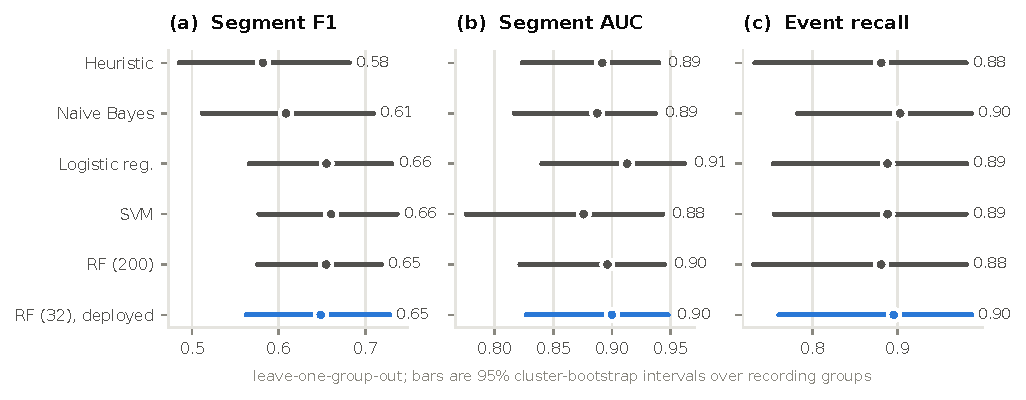
\includegraphics[width=\linewidth]{figures/fig_models.pdf}
\caption{Detection metrics under LOGO with 95\% cluster-bootstrap intervals. The deployed forest is highlighted. Intervals overlap for all learned models.\label{fig:models}}
\end{figure}

\textbf{Learned features do not help on this dataset.} Neither raw-window model beats the hand-crafted pipeline: ROCKET reaches segment F1 \R{abl.rocket.F1} (AUC \R{abl.rocket.AUC}) and the 1-D CNN \R{abl.cnn.F1} (AUC \R{abl.cnn.AUC}), against \R{abl.rfe.F1} (AUC \R{abl.rfe.AUC}) for the deployed forest; gradient boosting on the features is comparable to the forest (\R{abl.hgb.F1}, AUC \R{abl.hgb.AUC}). With \R{ds.poswindows}~positive windows, a model that must learn its own features has little to learn from.

\textbf{Ablations.} The rotation-invariant magnitude features alone (\R{fam.magnitudesonly.n} features) reach segment F1 \R{fam.magnitudesonly.F1} and AUC \R{fam.magnitudesonly.AUC}, and the \R{fam.gyromagnitudeonly.n} gyroscope-magnitude features alone reach \R{fam.gyromagnitudeonly.F1} and \R{fam.gyromagnitudeonly.AUC}---no worse than all \R{cfg.nfeat}. Accelerometer-only features are clearly weaker (F1 \R{fam.accelonly.F1}). A 2.1\,s window scored higher than the source study's 2.6\,s (F1 \R{win.2p1.F1} vs.\ \R{win.2p6.F1}) and longer windows were worse (3.6\,s: \R{win.3p6.F1}). These comparisons were made on the same LOGO folds that they are reported on and are hypothesis-generating; we did not change the shipped configuration on the strength of them, but they matter for Section~\ref{sec:robust}.

\textbf{Shift protocols.} Holding out a whole collection session or a whole Shimmer unit (Table~\ref{tab:shift}) leaves segment AUC essentially unchanged (deployed forest: \R{loso.rfe.segAUC} and \R{lodo.rfe.segAUC}, against \R{logo.rfe.segAUC} under LOGO) but moves event recall and specificity by several points in both directions. The heuristic keeps its recall under shift at the cost of much lower specificity (\R{loso.base.evSpec} under leave-one-session-out). Training on one Shimmer unit and testing on the other is the closest proxy the data offer for a change of hardware, and it costs the deployed forest event recall (\R{lodo.rfe.evRec} vs.\ \R{logo.rfe.evRec}).

\begin{table}[H]
\caption{Session and device shift. Leave-one-session-out holds out each of the three collection days; leave-one-device-out holds out each Shimmer3 unit.\label{tab:shift}}
\begin{adjustwidth}{-\extralength}{0cm}
\small
\begin{tabularx}{\fulllength}{lCCCCCCCC}
\toprule
 & \multicolumn{4}{c}{\textbf{Leave-one-session-out}} & \multicolumn{4}{c}{\textbf{Leave-one-device-out}}\\
\cmidrule(lr){2-5}\cmidrule(lr){6-9}
\textbf{Model} & \textbf{F1} & \textbf{AUC} & \textbf{Ev.\ rec.} & \textbf{Ev.\ spec.} & \textbf{F1} & \textbf{AUC} & \textbf{Ev.\ rec.} & \textbf{Ev.\ spec.}\\
\midrule
\inputtable{generated/tables/shift.tex}
\bottomrule
\end{tabularx}
\end{adjustwidth}
\end{table}

\subsection{The Verification Gate and Continuous Streams}
\label{sec:res-gate}
On curated events, the single-level sweep over \R{sweep.npolicies}~policies selects \R{single.rfe.policy} for the deployed forest, with event sensitivity \R{op.single.sens} and \R{op.single.far}\% false alarms per negative event (Figure~\ref{fig:gate}a). Requiring three votes caps sensitivity (best \R{sweep.bestsens.k3} at $K=3$ against \R{sweep.bestsens.k2} at $K=2$): the trained alert lasts about 2.5\,s, a window 2.6\,s, and at a 1.3\,s stride only two or three windows can be majority-spin.

\textbf{Nested selection.} Under nested selection the procedure chose \R{nest.rfe.npolicies} different policies across the \R{nest.rfe.nfolds}~outer folds (most often \R{nest.rfe.modal}, in \R{nest.rfe.modalcount} folds). Its out-of-sample event sensitivity is \R{nest.rfe.sens} (\R{nest.rfe.sensCI}) at \R{nest.rfe.far}\% (\R{nest.rfe.farCI}\%) false alarms per negative event, which slightly exceeds the 5\% bound the policy was selected to meet. Single-level selection was not optimistic here---the nested estimate is \R{nest.rfe.absdiff} \emph{higher} than the single-level one, well inside its interval---and the main thing nesting reveals is how unstable the selected policy is: with this little data, which policy wins depends on which recording is held out.

\textbf{Continuous streams.} Table~\ref{tab:streams} and Figure~\ref{fig:gate}b give the result that most changes the picture. Replaying whole recordings with held-out models and the nested policy, strict any-overlap scoring and no refractory period gives \R{cont.rfe.r0.fah}~FA/h (95\% exact interval \R{cont.rfe.r0.fahCI}) over \R{cont.rfe.r0.exposure}\,h of spin-free exposure---\R{cont.ratio.curated}$\times$ the \R{op.single.fah}~FA/h that the curated-event protocol implies for the same detector. The curated protocol omits exactly the motion where false alarms concentrate: its negative events are kept at least 1\,s from any spin and must fit whole between spins, so the approach to, and recovery from, a spin are never scored. Allowing a post-spin tolerance shows how much of the excess is boundary timing (Figure~\ref{fig:gate}b): with $\tau=10$\,s the rate falls to \R{cont.rfe.tol10.fah}~FA/h and with $\tau=20$\,s to \R{cont.rfe.tol20.fah}~FA/h---still roughly twice the curated estimate, so most of the gap is not a scoring artefact. With the 60\,s refractory period, \R{cont.rfe.r60.epdet} of \R{cont.rfe.r60.epn} alert episodes are detected (\R{cont.rfe.r60.epsens}, \R{cont.rfe.r60.epsensCI}) at \R{cont.rfe.r60.fah}~FA/h, with a median latency of \R{cont.rfe.r60.lat}\,s from the dog starting to spin.

On continuous streams the learned models' advantage largely disappears. The heuristic, also with a nested policy, detects \R{cont.base.r60.epsens} of episodes at \R{cont.base.r60.fah}~FA/h with the refractory period---indistinguishable from the forest at this sample size---although without the refractory period its false-alarm rate (\R{cont.base.r0.fah}~FA/h) is substantially higher than the forest's.

\begin{figure}[H]
\centering
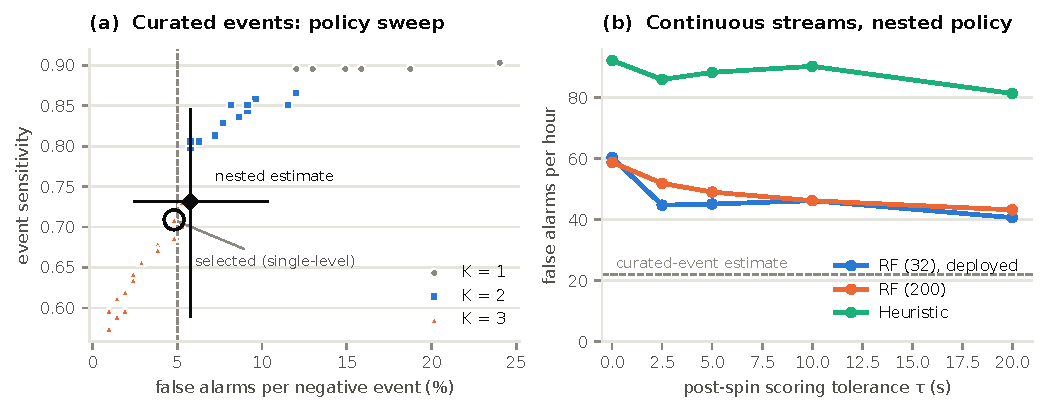
\includegraphics[width=\linewidth]{figures/fig_gate.pdf}
\caption{(\textbf{a}) The $K$-of-$N$ policy sweep on curated events for the deployed forest; the ring marks the single-level selection and the diamond the nested out-of-sample estimate with 95\% intervals. (\textbf{b}) False alarms per hour on continuous recordings as a function of the post-spin scoring tolerance $\tau$ (no refractory period, nested policy); the dashed line is the rate the curated protocol implies.\label{fig:gate}}
\end{figure}

\begin{table}[H]
\caption{Gate performance with nested policy selection: on curated events, and on continuous recordings with strict any-overlap scoring ($\tau=0$). Without the refractory period ($R=0$) every spin is a target; with $R=60$\,s spins closer than 60\,s form one episode. Intervals on FA/h are exact Poisson.\label{tab:streams}}
\begin{adjustwidth}{-\extralength}{0cm}
\small
\footnotesize
\begin{tabular}{lccccccc}
\toprule
 & \multicolumn{2}{c}{\textbf{Curated events}} & \multicolumn{2}{c}{\textbf{Stream, $R=0$}} & \multicolumn{3}{c}{\textbf{Stream, $R=60$\,s}}\\
\cmidrule(lr){2-3}\cmidrule(lr){4-5}\cmidrule(lr){6-8}
\textbf{Model} & \textbf{Sens.} & \textbf{FA/ev.\ (\%)} & \textbf{Spin sens.} & \textbf{FA/h} & \textbf{Ep.\ sens.} & \textbf{FA/h} & \textbf{Lat.\ (s)}\\
\midrule
\inputtable{generated/tables/streams.tex}
\bottomrule
\end{tabular}
\end{adjustwidth}
\end{table}

Figure~\ref{fig:timeline} shows one held-out recording end to end.

\begin{figure}[H]
\centering
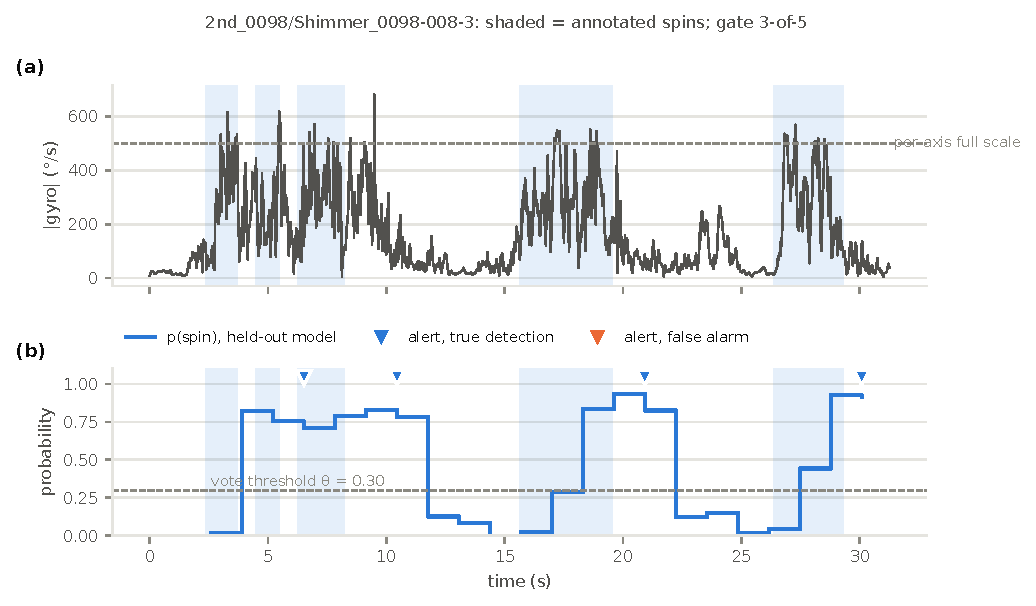
\includegraphics[width=\linewidth]{figures/fig_timeline.pdf}
\caption{One held-out recording (\TimelineRecording) as the collar would process it. (\textbf{a}) Gyroscope magnitude; shaded spans are annotated spins; the dashed line is the per-axis full scale at which the Shimmer3 saturates. (\textbf{b}) Window probabilities from a model that never saw this recording's group, the vote threshold, and the alerts the gate raises (refractory period off for visibility).\label{fig:timeline}}
\end{figure}

\subsection{Formal Verification of the Escalation Protocol}
\label{sec:formal-results}
Table~\ref{tab:tlc} lists the \R{tlc.nchecks} TLC checks (\R{tlc.nwitness} of which are reachability witnesses, omitted from the table, all violated as required). Every check came out as expected. For the system as built, every safety property of the ladder itself holds under arbitrary owner and caregiver behaviour, relay death and network partitions: no channel is paged twice; the relay pages the emergency contact only after $T_1+T_2$ (or $T_1$ with no caregiver configured); the relay never escalates after the owner responded; with a live relay every alert closes by $T_1+T_2$; if the backend ever learned of the alert, it closes within $T_1+T_2+W+1$ ticks even if the relay dies; and terminal states absorb. With a reliable phone and network, the three end-to-end properties also hold.

Under faults, TLC produced counterexamples to three properties, each of which is a real behaviour of the design:

\begin{enumerate}
\item \textbf{The watchdog skips the caregiver tier.} In the shortest counterexample (Appendix~\ref{app:cex}) the phone dies one tick after mirroring the alert. The backend sees an open alert and no heartbeats, and the Direct watchdog pages the emergency contact at tick \R{tlc.premature.tick} (\R{tlc.premature.s}\,s)---before the caregiver would have been paged at $T_1$---and, the phone being dead, the caregiver is never paged at all. A network partition produces the same premature page while the relay is still alive; the relay then escalates on its own as well, and the emergency contact is paged twice (the \texttt{AtMostOneEmergencyPage} counterexample).
\item \textbf{A lost acknowledgement causes an emergency page.} The owner acknowledges; the phone dies before mirroring that to the backend; the watchdog sees an open alert with a silent relay and escalates. This is the designed ``err towards escalating'' behaviour, and model checking makes its cost explicit.
\item \textbf{An alert can be lost silently.} If the network is down when the gate fires and the phone dies before it reconnects, the backend never learns of the alert and nobody beyond the owner's dead phone is ever told. No backend design can repair this; only a second path from the collar can.
\end{enumerate}

The \emph{Ladder} watchdog removes the first defect. It is verified never to page the emergency contact before $T_1+T_2$, preserves at-most-once paging by each party and the bounded-response guarantee, and can still reach the emergency contact; duplicate pages between relay and backend under a partition remain possible and require idempotent paging at a shared provider.

\begin{table}[H]
\caption{TLC results (reachability witnesses omitted). ``Reliable'': phone never dies and network never partitions; ``faults'': both may happen at any time. Direct: watchdog as built; Ladder: proposed variant.\label{tab:tlc}}
\small
\begin{tabularx}{\textwidth}{>{\raggedright\arraybackslash}Xlllr}
\toprule
\textbf{Property} & \textbf{Model} & \textbf{Watchdog} & \textbf{Verdict} & \textbf{States}\\
\midrule
\inputtable{generated/tables/tlc.tex}
\bottomrule
\end{tabularx}
\end{table}

\textbf{Conformance and an integration defect.} The property-based tests found no disagreement between the shipped engine and the model's invariants in \R{prop.examples}~random executions per property. Writing the model, however, required stating precisely how the backend associates heartbeats with alerts---and the code did it inconsistently: the relay labelled heartbeats with the \emph{owner's} contact identifier while the watchdog matched them against the alert's \emph{dog} identifier. The two never matched, so in deployment the watchdog would have treated every relay as one that had never heartbeated and would have fallen back to its 600\,s ceiling. Every unit test passed with the bug present, because each side was tested against its own fixtures. We fixed it and added a regression test.

\subsection{End-to-End Outcomes}
\label{sec:sim-results}
With the measured detector (episode sensitivity \R{sim.pdetect}), the dominant loss in every scenario is the alert that is never detected (Figure~\ref{fig:sim}a). When the owner is incapacitated, a human responds within 300\,s in \R{sim.ownerincapacitated.p300}\% of episodes (median \R{sim.ownerincapacitated.median}\,s among those reached), and the ladder delivers that response in \R{sim.ownerincapacitated.p300givendet}\% of the episodes the collar detects. If the dog repeats an unacknowledged alert up to three times, 30\,s apart, detection rises to \R{sim.rep3.pdet}\% and the 300\,s figure to \R{sim.rep3.p300}\%, at the cost of a later median (\R{sim.rep3.median}\,s). Whether trained dogs repeat in this way is not in the dataset, and it is the single largest lever on outcomes available without better sensing. When the owner is awake, \R{sim.ownerawake.byowner}\% of episodes are closed by the owner and only \R{sim.ownerawake.care}\% reach the caregiver; asleep, \R{sim.ownerasleep.care}\% do.

Fault injection reproduces the model-checking findings quantitatively (Figure~\ref{fig:sim}b). With the phone dying at a random time in the first 240\,s while the owner is incapacitated, the Direct watchdog skips the caregiver tier in \R{sim.incapacitatedrelaydies.skipped}\% of episodes; the Ladder watchdog in \R{sim.incapacitatedrelaydies.ladder.skipped}\%. Under partitions, duplicate emergency pages occur in \R{sim.incapacitatedpartition.dup}\% of episodes with the Direct watchdog and \R{sim.incapacitatedpartition.ladder.dup}\% with the Ladder watchdog, and with an awake owner \R{sim.awakepartition.afterack}\% of episodes page someone after the owner has already responded. Alerts lost because the phone died before the backend heard of them occur in \R{sim.incapacitatedrelaydies.lost}\% of those stress episodes. The sensitivity analysis over the asleep-owner assumptions is informative mainly about speed. Within 300\,s the monitoring tier catches nearly every detected episode that owner and caregiver miss, so that figure moves only between \R{tornado.p300.min}\% and \R{tornado.p300.max}\% across all variations---it is governed by detection, not by the humans. Within 180\,s it ranges from \R{tornado.p180.min}\% to \R{tornado.p180.max}\%, most strongly with caregiver availability (\R{tornado.care.lo}\% at \R{tornado.care.vlo} to \R{tornado.care.hi}\% at \R{tornado.care.vhi}) and caregiver response time (\R{tornado.caremed.lo}\% at a \R{tornado.caremed.vlo}\,s median to \R{tornado.caremed.hi}\% at \R{tornado.caremed.vhi}\,s).

\begin{figure}[H]
\centering
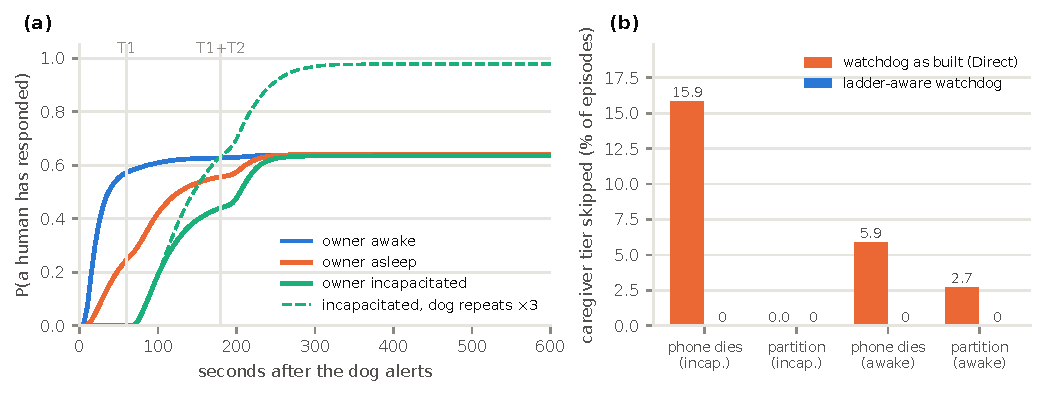
\includegraphics[width=\linewidth]{figures/fig_sim.pdf}
\caption{(\textbf{a}) Probability that a human has responded, by time after the dog alerts, for three owner states and for an incapacitated owner whose dog repeats an unacknowledged alert. The curves plateau below 1 because undetected alerts never start the ladder. (\textbf{b}) Share of episodes in which the emergency contact is paged before any caregiver page, under injected faults, for the watchdog as built and the ladder-aware variant.\label{fig:sim}}
\end{figure}

\textbf{False-alarm burden and the requirement it implies.} With the shipped timings and the assumed owner behaviour, \R{burden.preach}\% of false alarms reach the caregiver: the owner-acknowledgement stage attenuates false alarms by a factor of \R{burden.attenuation} before they reach anyone else. That is not enough. At the measured training-session rate of \R{burden.measured.fah}~FA/h a caregiver would be paged about \R{burden.measured.careday} times a day. Inverting Equation~(\ref{eq:burden}) for one caregiver page per week requires a detector false-alarm rate of at most \R{req.maxfah}~FA/h (\R{req.maxfaday} per day; Figure~\ref{fig:burden}a)---\R{req.factor}$\times$ below the measured rate, and of the same order as the 0.2--2.5 false alarms per day of clinically validated seizure wearables~\cite{naganur2022meta,meritamlarsen2023nonEEG}. One emergency page per month requires \R{req.maxfahemerg}~FA/h. The timing grid (Figure~\ref{fig:burden}b) shows the trade-off the ladder can offer on top of this: shortening $T_1$ to 30\,s raises the probability of help within 180\,s for an incapacitated owner but lets \R{grid.t1short.preach}\% of false alarms through to the caregiver, against \R{burden.preach}\% at 60\,s and \R{grid.t1long.preach}\% at 120\,s.

\begin{figure}[H]
\centering
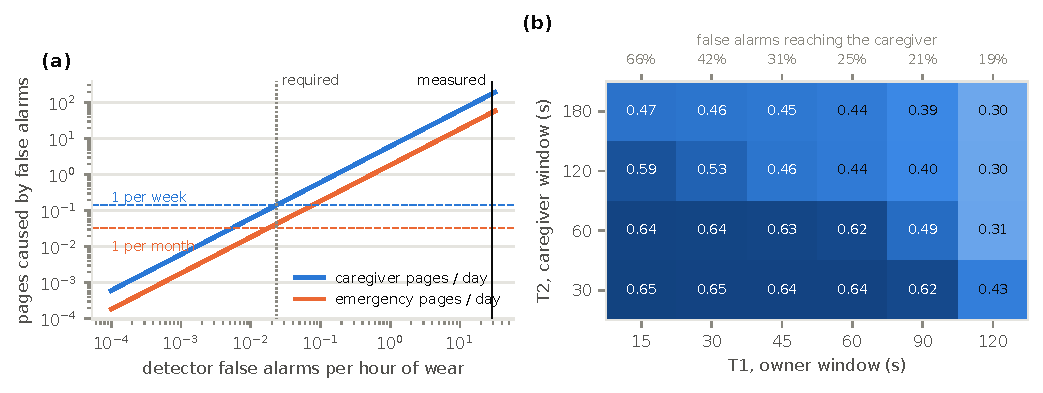
\includegraphics[width=\linewidth]{figures/fig_burden.pdf}
\caption{(\textbf{a}) Pages caused by false alarms alone as a function of the detector's false-alarm rate, with the shipped $T_1=60$\,s and $T_2=120$\,s; the vertical lines mark the measured training-session rate and the rate that keeps caregiver pages to one per week. (\textbf{b}) Probability that a human responds within 180\,s when the owner is incapacitated, over the $(T_1, T_2)$ grid; the top axis gives the share of false alarms that reach the caregiver for each $T_1$.\label{fig:burden}}
\end{figure}

\subsection{Embedded Implementation and Sensor Transfer}
\label{sec:robust}
The transpiled forest (\R{fw.trees}~trees, \R{fw.nodes}~nodes, \R{fw.kib}\,KiB) agrees with scikit-learn to \R{fw.transpile} in probability; the complete C pipeline, from raw window to probability, agrees with the Python pipeline to \R{fw.probaerr} on \R{fw.windows}~real windows, with worst feature relative error \R{fw.featerr}, and passes all \R{fw.checks}~host checks. The size/accuracy front over \R{front.n}~forest configurations (Figure~\ref{fig:front}) is flat: segment AUC spans only \R{front.aucmin}--\R{front.aucmax}, and \R{front.small.trees}~trees of depth \R{front.small.depth} (\R{front.small.kib}\,KiB) come within 0.01 AUC of the shipped forest. On the host, one window costs \R{bench.us}\,$\mu$s with the twiddle-table DFT against \R{bench.direct.us}\,$\mu$s with in-loop \texttt{sinf}/\texttt{cosf} (\R{bench.trig}~transcendental calls per window); the forest walk visits \R{bench.visits}~nodes. We have not measured the cost on an ESP32 and report no estimate of it.

\begin{figure}[H]
\centering
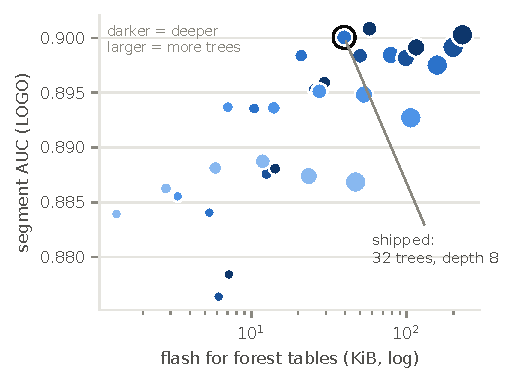
\includegraphics[width=0.62\linewidth]{figures/fig_front.pdf}
\caption{Segment AUC against flash footprint for \R{front.n} forest configurations (4--128 trees, depth 4--12) under LOGO.\label{fig:front}}
\end{figure}

\textbf{Transfer to the MPU6050.} Passing held-out windows through the datasheet's noise, offset and sensitivity errors and 16-bit quantisation leaves event recall unchanged (\R{rob.c.mpu6050datasheet.evRec} vs.\ \R{rob.c.clean.evRec}; Figure~\ref{fig:robust}), as do 5\,ms sampling jitter and a 50\,Hz rather than 51.2\,Hz collar. Range does matter: restricting the gyroscope to a 250\,\textdegree{}/s full scale---the MPU6050's power-on default---drops event recall to \R{rob.c.gyrofullscale250dps.evRec}, whereas the $\pm$2000\,\textdegree{}/s range the firmware configures loses nothing (and a 45\,Hz collar costs little, \R{rob.c.rate45hz.evRec}). \textbf{Collar rotation is the dominant risk.} A 90\textdegree{} rotation about the device $x$ axis drops event recall to \R{rob.c.rotx90deg.evRec}, and about $z$ to \R{rob.c.rotz90deg.evRec}; a uniformly random orientation to \R{rob.c.rotrandomso3.evRec}. Training with two randomly rotated copies of every window restores recall (\R{rob.a.rotrandomso3.evRec} under random rotation) at a small cost on unrotated data (\R{rob.a.clean.evRec}), and the magnitude-only model is invariant by construction: its event recall is \R{rob.m.rotrandomso3.evRec} under every rotation, slightly below the unrotated full model's \R{rob.c.clean.evRec}. Because a collar does rotate around the neck between fittings, we recommend one of the two for any physical deployment.

\begin{figure}[H]
\centering
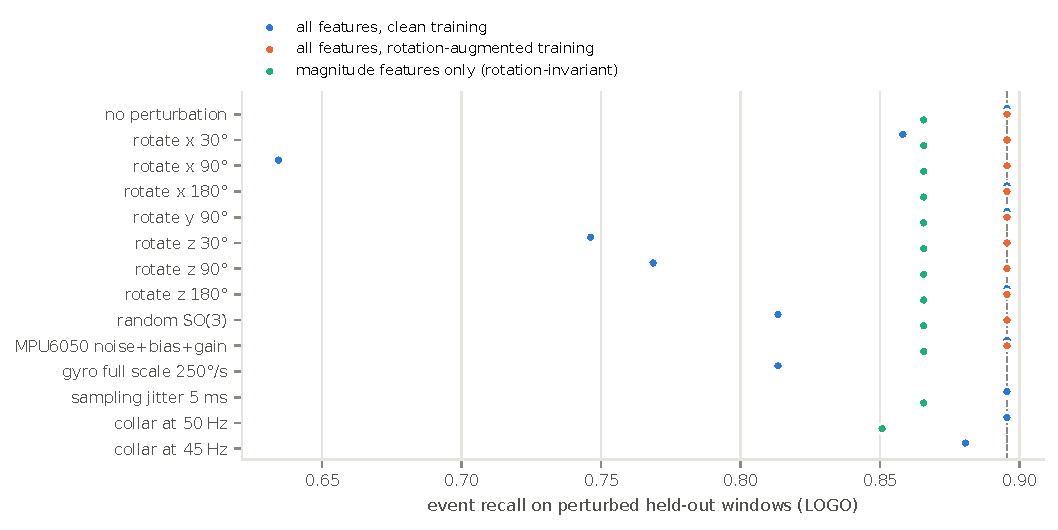
\includegraphics[width=\linewidth]{figures/fig_robustness.pdf}
\caption{Event recall of the deployed configuration on held-out windows under simulated sensor-transfer perturbations, for clean training, rotation-augmented training, and a model restricted to rotation-invariant magnitude features. The dashed line is unperturbed performance.\label{fig:robust}}
\end{figure}
